%! Author = stefano
%! Date = 22/11/2020

% Preamble
\documentclass[11pt]{article}
\usepackage[utf8]{inputenc}
\usepackage{dirtree}
\usepackage{graphicx}
\graphicspath{ {../images/} }

\title{Pedestrian Intent Prediction}
\author{Stefano Zanatta, Pasquale Coscia, Lamberto Ballan}
\date{\today}

% Packages
\usepackage{amsmath}
\usepackage{hyperref}

% Document
\begin{document}
\maketitle
\section{Introduction}
    We implemented the work of Haziq Razali, Alexandre Alah:
    Pedestrian-Intention-Prediction\footnote{\url{https://github.com/lucyze/Pedestrian-Intention-Prediction}}.
    The original work consists in a Convolutional Neural Network - LSTM, with the goal to predict the intention
    of pedestrians on crossing the road.\\
    The model was originally trained on Lausanne Dataset (not public) and on JAAD Dataset\footnote{\url{http://data.nvision2.eecs.yorku.ca/JAAD_dataset/}}.
    The former was recorded by static cameras, the latter on moving cameras (placed in the cars).\\
    The goal of this project is to study the pipeline, reproduce the experiments on the JAAD dataset, then adapt and
    improve the model for the PIE dataset\footnote{\url{https://data.nvision2.eecs.yorku.ca/PIE_dataset/}}.

\section{Lausanne Dataset}
    %TODO general results on lausanne (by Haziq Razali)

\section{JAAD Dataset}
    The JAAD datasets consists of mp4 videos, each one associated to a rich description, frame to frame, of what is happening on a given moment:
    \begin{itemize}
        \item id of the pedestrian
        \item coordinates of the pedestrian on the relative frame
        \item standing, walking
        \item looking at the traffic
        \item hand gesture
        \item speeding up/slowing down
        \item crossing the road
        \item occlusion
    \end{itemize}
    For the target we only use the information about crossing the road.\\
    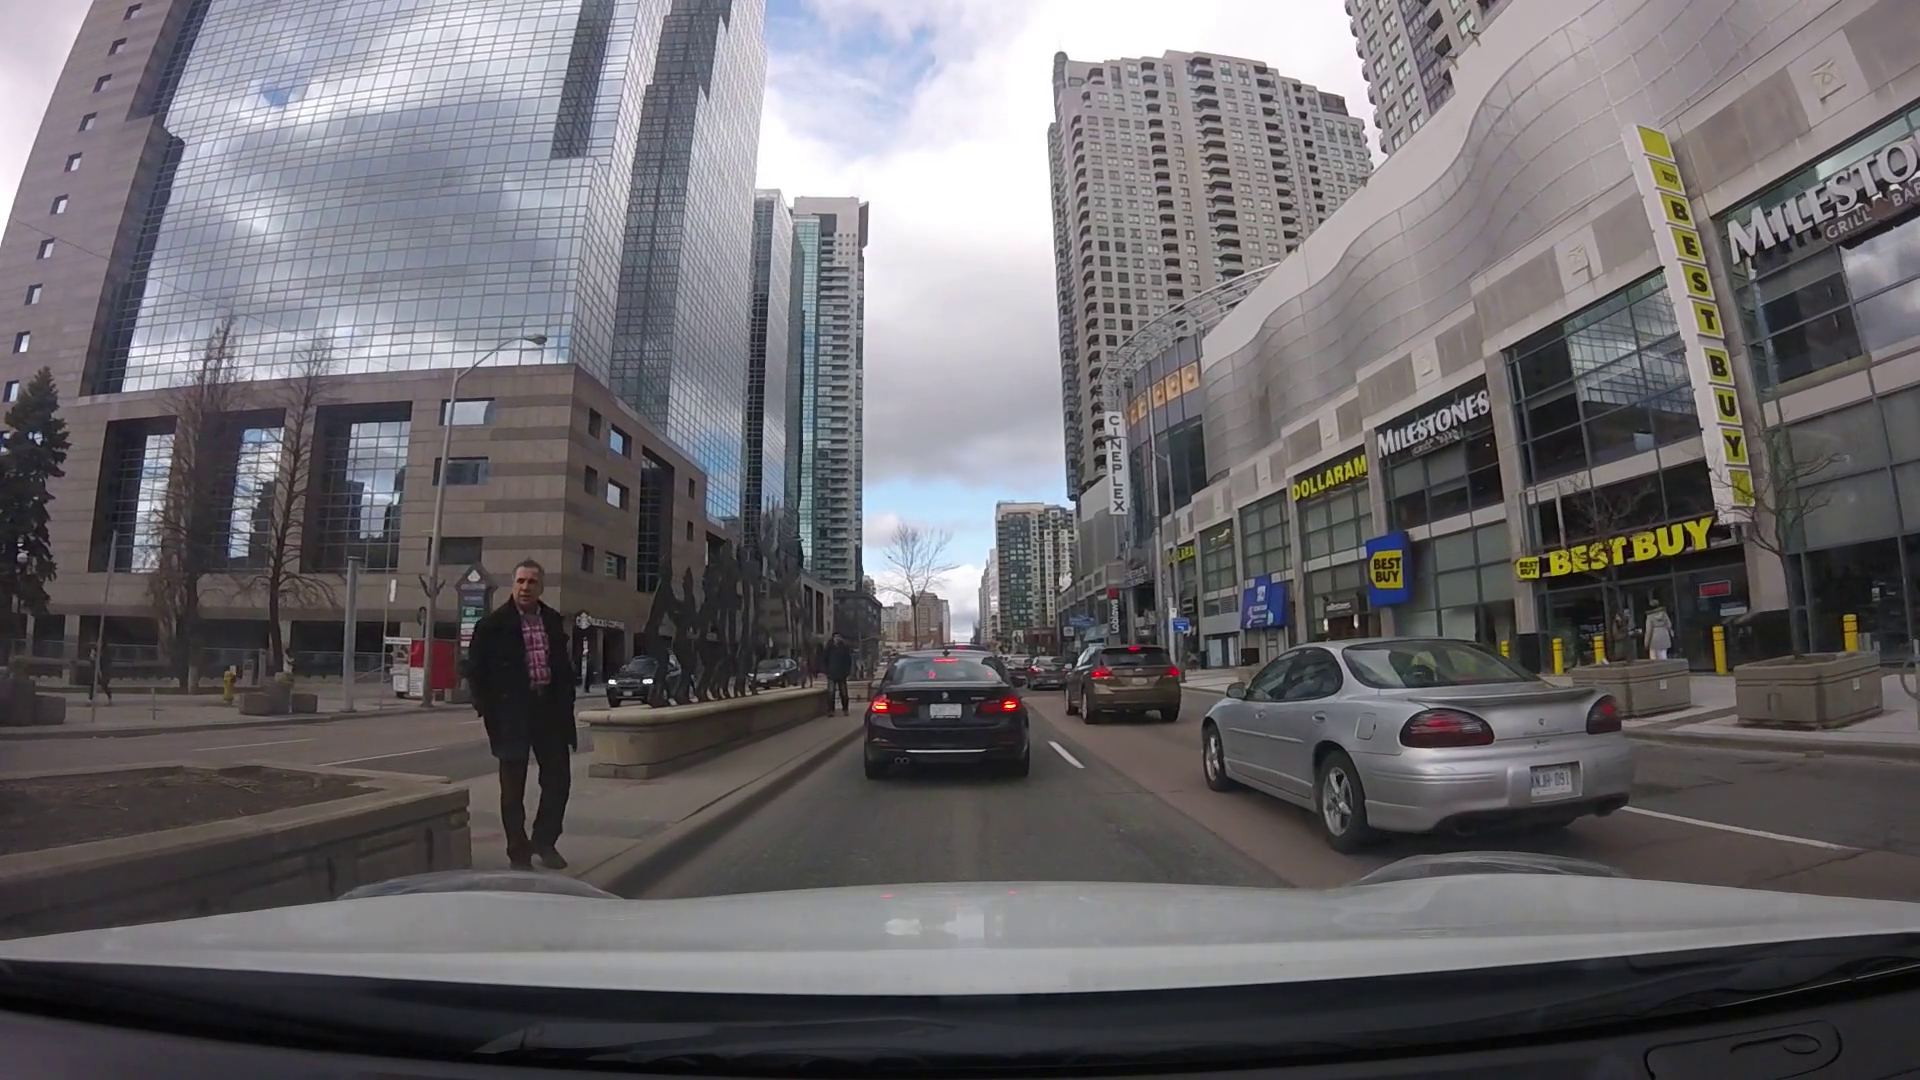
\includegraphics[width=\textwidth]{jaadscene}\\

\section{Pipeline}
\subsection*{Adapting the ground truth}
    The first step is to create the ground truth for the model by transforming the input into a csv.
    Originally, the Lausanne dataset required a step to locate the pedestrians (with an external object detector)
    and the (static) coordinates of the road.
    This is not longer required, because JAAD and PIE include the coordinates of the pedestrians and whether or not
    they are crossing the road.
    \begin{center}
    \begin{tabular}{ c c c c c c c c c c}
     frame & id & tlx & tly & width & height & walking & standing & looking & incrossing\\
     1,0 & 463 & 730 & 69 & 118 & 0 & 1 & 0 & 0 & 0\\
     1,0 & 463 & 730 & 69 & 118 & 0 & 1 & 0 & 0 & 1\\
    \end{tabular}
    \end{center}
\subsection*{Trajectories}
    The second Step consists in assigning, at each frame, the ``lifetime'' of the pedestrian in the video, and a ``cross'' column, indicating if they
    ever crossed the road in their lifetime.
    \begin{center}
    \begin{tabular}{ c c c}
     incrossing & lifetime & cross\\
     0 & 568 & 0\\
     0 & 568 & 0\\
    \end{tabular}
    \end{center}
\subsection*{Hungarian Tracker}
    Remove pedestrians with a lifetime below a threshold, and change pedestrians IDs to a numeric value.
\subsection*{Crop Pedestrians}
    Crops each pedestrian into images, organized in sub-folders:
    \dirtree{%
        .1 dataset.
        .2 all.
        .3 crops.
        .4 name\_of\_the\_video.
        .5 id\_of\_the\_pedestrian.
        .6 id\_pedestrian\_png.
    }\\
    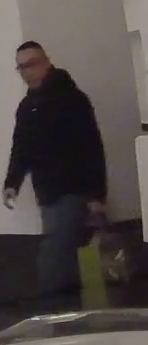
\includegraphics[width=0.4\textwidth]{crop}\\
    Then appends the path of the crop to each frame's annotation.
    \begin{center}
    \begin{tabular}{ c c c c c c c c c c c c c c}
     filename & folderpath\\
     00000001.png & crops\video\_0001\0000000000\\
     00000001.png & crops\video\_0001\0000000000\\
    \end{tabular}
    \end{center}
\subsection*{Save Scenes}
    Add the whole scenes to the dataset and adds their paths to the annotations.
    \dirtree{%
        .1 dataset.
        .2 all.
        .3 scenes.
        .4 name\_of\_the\_video.
        .5 id\_video\_png.
    }
    The new annotations columns are:
    \begin{center}
    \begin{tabular}{ c c }
     scene\_filename & scene\_folderpath \\
     00000001.png & scenes\video\_0001 \\
     00000001.png & scenes\video\_0001 \\
    \end{tabular}
    \end{center}

\subsection*{Split train test}
    In the last step the dataset is split into train and test:
    \dirtree{%
    .1 dataset.
    .2 train.
    }\\
    \dirtree{%
    .1 dataset.
    .2 test.
    }
\section{Model}
The model is composed of a VGG-16 pre trained CNN, a fully connecter layer (feature embedder), a LSTM and
a linear classifier to predict if the pedestrian crossed the road.\\
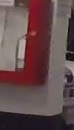
\includegraphics[width=0.4\textwidth]{jaaderrorcrop}\\

\subsection*{VGG-16}
This is a pre-trained CNN that works as a feature extractor for each image.
This operation is executed for each image in the batch.
\subsection*{Feature Embedder}
Embed the CNN output into a 255 units vector.
Then perform dropout.

\subsection*{LSTM}
Process the sequence through the LSTM with ReLU activation function and dropout.


\subsection*{Linear Classifier}
Classify whether the pedestrian crossed the road or not.

\subsection*{Changes to the original model}
To improve the results, we added the entire scene as input for the prediction.
We added a new CNN, followed by a LSTM to create the sequence, then we merged the scene-LSTM output with the crops-LSTM
outputs and adapted the input size of the linear predictor.

\\
Another change was to add more actions as target for the linear predictor.
This makes the task harder, but should make the model more robust to overfitting.


\section{PIE Dataset}
\#todo

\section{PIE Pipeline}
\#todo


\section{Results}
    The model works best when there is a clear distinction between the pedestrians are not-crossing (for their initial lifetime)
    and crossing the road (at the end of their lifetime).
    It works poorly for large roads where the same pedestrians can move in and out the road repeatedly.\\
    The original experiments where done on datasets where the direction of movement of the pedestrians where already known.
    For the Jaad dataset, instead, the directions were unkown and the results were much worse.
    \includegraphics[width=\textwidth]{results_original}\\

\end{document}


[train] best accuracy at lowest loss  0.9405099150141643
[train] best accuracy at highest accuracy  0.9405099150141643
[val] best accuracy at lowest loss  0.6571428571428571
[val] best accuracy at highest accuracy  0.7142857142857143


[INFO: train.py:  234]:   [val] d_accuracy: 0.629
[INFO: train.py:  234]:   [val] d_fn: 14.000
[INFO: train.py:  234]:   [val] d_fp: 12.000
[INFO: train.py:  234]:   [val] d_loss: 1.138
[INFO: train.py:  234]:   [val] d_precision: 0.707
[INFO: train.py:  234]:   [val] d_recall: 0.674
[INFO: train.py:  234]:   [val] d_tn: 15.000
[INFO: train.py:  234]:   [val] d_tp: 29.000
[INFO: train.py:  237]:   [train] d_accuracy: 0.941
[INFO: train.py:  237]:   [train] d_fn: 5.000
[INFO: train.py:  237]:   [train] d_fp: 16.000
[INFO: train.py:  237]:   [train] d_loss: 0.178
[INFO: train.py:  237]:   [train] d_precision: 0.927
[INFO: train.py:  237]:   [train] d_recall: 0.976
[INFO: train.py:  237]:   [train] d_tn: 128.000
[INFO: train.py:  237]:   [train] d_tp: 204.000

(on gpu)
[INFO: train.py:  234]:   [val] d_accuracy: 0.614
[INFO: train.py:  234]:   [val] d_fn: 19.000
[INFO: train.py:  234]:   [val] d_fp: 8.000
[INFO: train.py:  234]:   [val] d_loss: 1.147
[INFO: train.py:  234]:   [val] d_precision: 0.750
[INFO: train.py:  234]:   [val] d_recall: 0.558
[INFO: train.py:  234]:   [val] d_tn: 19.000
[INFO: train.py:  234]:   [val] d_tp: 24.000
[INFO: train.py:  237]:   [train] d_accuracy: 0.955
[INFO: train.py:  237]:   [train] d_fn: 12.000
[INFO: train.py:  237]:   [train] d_fp: 4.000
[INFO: train.py:  237]:   [train] d_loss: 0.153
[INFO: train.py:  237]:   [train] d_precision: 0.980
[INFO: train.py:  237]:   [train] d_recall: 0.943
[INFO: train.py:  237]:   [train] d_tn: 140.000
[INFO: train.py:  237]:   [train] d_tp: 197.000
[INFO: train.py:  258]: Saving checkpoint to ./models/cnnlstm_jaad_standardcrop_with_model.pt
[INFO: train.py:  260]: Done.
[train] best accuracy at lowest loss  0.9490084985835694
[train] best accuracy at highest accuracy  0.9546742209631728
[val] best accuracy at lowest loss  0.6714285714285714
[val] best accuracy at highest accuracy  0.6714285714285714


(+scenes on gpu)
[INFO: train-scenes.py:  234]:   [val] d_accuracy: 0.600
[INFO: train-scenes.py:  234]:   [val] d_fn: 20.000
[INFO: train-scenes.py:  234]:   [val] d_fp: 8.000
[INFO: train-scenes.py:  234]:   [val] d_loss: 1.190
[INFO: train-scenes.py:  234]:   [val] d_precision: 0.742
[INFO: train-scenes.py:  234]:   [val] d_recall: 0.535
[INFO: train-scenes.py:  234]:   [val] d_tn: 19.000
[INFO: train-scenes.py:  234]:   [val] d_tp: 23.000
[INFO: train-scenes.py:  237]:   [train] d_accuracy: 0.977
[INFO: train-scenes.py:  237]:   [train] d_fn: 7.000
[INFO: train-scenes.py:  237]:   [train] d_fp: 1.000
[INFO: train-scenes.py:  237]:   [train] d_loss: 0.104
[INFO: train-scenes.py:  237]:   [train] d_precision: 0.995
[INFO: train-scenes.py:  237]:   [train] d_recall: 0.967
[INFO: train-scenes.py:  237]:   [train] d_tn: 143.000
[INFO: train-scenes.py:  237]:   [train] d_tp: 202.000
[INFO: train-scenes.py:  258]: Saving checkpoint to ./models/cnnlstm_jaad_standardcrop_with_model.pt
[INFO: train-scenes.py:  260]: Done.
[train] best accuracy at lowest loss  0.9773371104815864
[train] best accuracy at highest accuracy  0.9773371104815864
[val] best accuracy at lowest loss  0.6428571428571429
[val] best accuracy at highest accuracy  0.7428571428571429
